\section{电磁感应与电磁波}
\gdef\coursepart{电磁感应与电磁波}

\begin{frame}{电磁感应与电磁波}
电磁感应是磁通变化时回路中产生电动势的现象；电磁波是变化的电场与磁场相互激发、在空间中传播的波。
基本性质：法拉第电磁感应定律（动生与感生），位移电流（变化的电场进入安培环路）。与两个高斯定律合在一起，写成麦克斯韦方程组。

几类电磁感应与电磁波问题的一般方法：\\
（1）电动势：动生用 $\vct v\times\vct B$，感生用法拉第定律\\
（2）电路问题：自感、互感、磁场能量与 $RL$ 暂态\\
（3）位移电流补进安培环路，写成麦克斯韦方程组，和边值关系一并求解\\
（4）能动量：坡印廷矢量，动量和角动量守恒\\
（5）电磁波：波动方程与平面波，界面上求反射和折射
\src{张讲义第八、九章；DC7、DC8、DC10；缪讲义电磁感应、位移电流与电磁波。}
\end{frame}

\begin{frame}{动生电动势}
导体相对磁场运动时，其中的载流子受到洛伦兹力。单位正电荷受到的力是 $\vct v\times\vct B$，方向和大小都与静电场力 $\vct E$ 相同，所以把它看成等效电场。
\[
 \mathcal{E}=\int(\vct v\times\vct B)\cdot\dd\vct l.
\]
$\vct v$ 是导体上该点相对磁场的速度，$\dd\vct l$ 沿导线从一端指向另一端。$\vct v$ 与 $\vct B$ 平行的一段，贡献为零。

开路时，电荷移到两端，静电场与 $\vct v\times\vct B$ 平衡，两端电势差等于这个电动势。闭合时，电流等于电动势除以回路电阻。

直杆长 $\ell$，在均匀磁场里平动，并且 $\vct v$、$\vct B$、杆三者两两垂直时，$\mathcal{E}=B\ell v$。速度或磁场沿杆不均匀时，必须沿杆积分。
\src{张讲义第8.1--8.2节，式(8.7)--(8.9)；DC7，动生电动势。}
\end{frame}

\begin{frame}{感生电动势}
磁场随时间变化时，空间中产生感生电场。它沿闭合曲线的积分一般不为零：
\[
 \oint_C\vct E\cdot\dd\vct l
 =-\frac{\dd\Phi_B}{\dd t}
 =-\int_S\frac{\partial\vct B}{\partial t}\cdot\dd\vct S.
\]
感生电场不是保守场，有旋度，不能写成某个电势的梯度。

回路正向和曲面法向成右手关系。负号表示感应电流自己产生的磁通，阻碍引起感应的那个磁通变化。

一般会利用对称性把 $E$ 从积分号里提出来计算
\src{张讲义第8.2节，式(8.13)、(8.23)；DC7，感生电场。}
\end{frame}

\begin{frame}{电动势}
合并动生和感生两种电动势，有：
\[
 \boxed{\mathcal{E}
 =\oint_C(\vct E+\vct v\times\vct B)\cdot\dd\vct l
 =-\frac{\dd\Phi_B}{\dd t}}.
\]
$\vct E$ 是感生电场，$\vct v\times\vct B$ 是运动导体里的等效电场。右边是回路所围磁通的变化率。

\src{张讲义式(8.9)、(8.13)、(8.23)；DC7。}
\end{frame}

\begin{frame}{滑动导体杆}
\begin{columns}[T,onlytextwidth]
\begin{column}{0.34\textwidth}
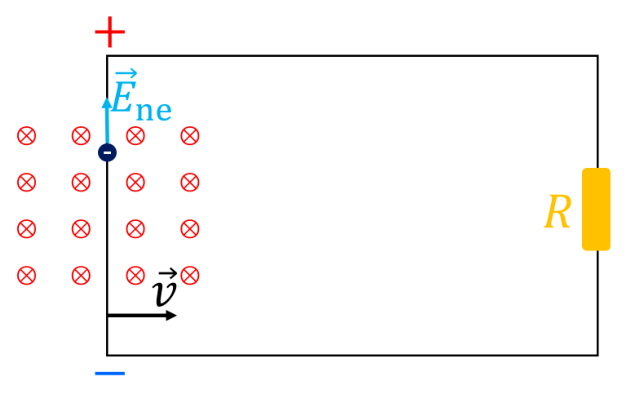
\includegraphics[width=\linewidth]{m3_sliding_rod.png}

杆长 $\ell$，速度 $v$ 向右。磁场垂直纸面向内，回路电阻为 $R$。
\end{column}
\begin{column}{0.62\textwidth}
等效电场 $\vct v\times\vct B$ 向上，
\[
 \mathcal{E}=B\ell v.
\]
上端电势高，电流沿顺时针方向。
\[
 I=\frac{B\ell v}{R},\qquad
 F_B=\frac{B^2\ell^2}{R}v.
\]
磁力向左，阻碍杆向右运动。匀速时外力向右，外力的功率等于焦耳热：
\[
 F_{\rm ext}v=\mathcal{E}I=I^2R.
\]
\end{column}
\end{columns}
磁力始终垂直于载流子的总速度，不对载流子做功。焦耳热来自外力。撤去外力后
\[
 m\dot v=-\frac{B^2\ell^2}{R}v,\qquad
 v=v_0\e^{-t/\tau},\qquad
 \tau=\frac{mR}{B^2\ell^2}.
\]
这里忽略了自感，电流随速度立刻变化。
\src{张讲义发电机原理；DC7；缪讲义磁阻尼。}
\end{frame}

\begin{frame}{圆形磁场}
\begin{columns}[T,onlytextwidth]
\begin{column}{0.28\textwidth}
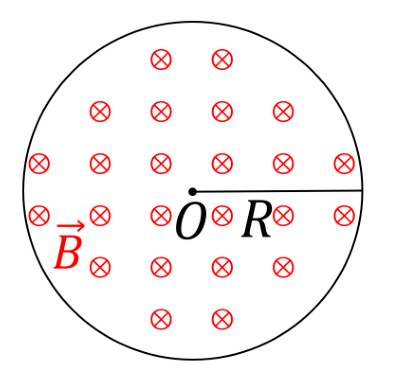
\includegraphics[width=\linewidth]{m3_finite_B.png}

磁场局限在半径 $R$ 的圆柱内，方向垂直纸面。
\end{column}
\begin{column}{0.68\textwidth}
$B_z(t)$ 以向外为正，感生电场 $E_\varphi$ 以逆时针为正。$r<R$ 时，回路围住的磁通是 $\pi r^2B_z$，
\[
 E_\varphi=-\frac{r}{2}\dot B_z.
\]
$r>R$ 时，磁通只来自半径 $R$ 以内，
\[
 E_\varphi=-\frac{R^2}{2r}\dot B_z.
\]
\end{column}
\end{columns}
$E_\varphi$ 在 $r=R$ 连续。区内随 $r$ 增大，区外按 $1/r$ 减小。区外 $B=0$，环路围住的磁通仍在变化，所以仍有感生电场。$\dot B_z>0$ 时电场沿顺时针方向。
\src{张讲义例8.3；DC7例3。}
\end{frame}

\begin{frame}{涡流}
导体盘半径 $a$、厚度 $\delta$、电导率 $\sigma$。磁场只在 $r\le R$ 内不为零，且 $R<a$，那里 $B_z=B_0(t)$。忽略涡流对这个外加磁场的反作用。

感生电场就是圆形磁区的结果，$\vct J=\sigma E_\varphi\vct e_\varphi$。焦耳热功率密度为 $\sigma E_\varphi^2$。薄环体积 $2\pi r\delta\,\dd r$，分内外两段积分：
\[
 \begin{aligned}
 P&=2\pi\delta\sigma\dot B_0^{\,2}
 \left(\int_0^R\frac{r^3}{4}\,\dd r
 +\int_R^a\frac{R^4}{4r}\,\dd r\right)\\
 &=\boxed{\dfrac{\pi\delta\sigma R^4}{8}\dot B_0^{\,2}
 \left(1+4\ln\frac{a}{R}\right)}.
 \end{aligned}
\]
括号里第一项来自磁区内部，对数项来自外部环形导体。只改变外半径 $a$ 时，变的是第二项。

这个算法要求外加 $B_0(t)$ 已知。涡流很强、足以改变磁通时，要先把反作用算进 $B$。
\src{期中复习笔记题7.6；缪讲义6.2；DC7涡流。}
\end{frame}

\begin{frame}{旋转圆盘}
\begin{columns}[T,onlytextwidth]
\begin{column}{0.30\textwidth}
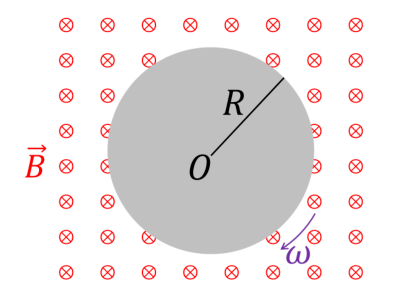
\includegraphics[width=\linewidth]{m3_rotating_disk.png}

半径 $R$ 的导体盘绕轴转动，均匀磁场垂直盘面。图中 $\vct\omega$ 与 $\vct B$ 同向。
\end{column}
\begin{column}{0.66\textwidth}
距轴 $s$ 处速度为 $\omega s$，正电荷受力沿径向向外。中心到边缘
\[
 \mathcal{E}
 =\int_0^R\omega s B\,\dd s
 =\frac12 B\omega R^2.
\]
开路达到平衡时，$\vct E+\vct v\times\vct B=0$，边缘电势比中心高 $\dfrac12 B\omega R^2$。电刷接通中心和边缘后，回路里才有持续电流。
\end{column}
\end{columns}
盘的面积不变，总磁通也不变。中心到边缘是开路，电动势沿半径对 $\vct v\times\vct B$ 积分。
\src{张讲义例8.1；DC7动生电动势。}
\end{frame}

\begin{frame}{电磁刹车}
\begin{columns}[T,onlytextwidth]
\begin{column}{0.30\textwidth}
\centering
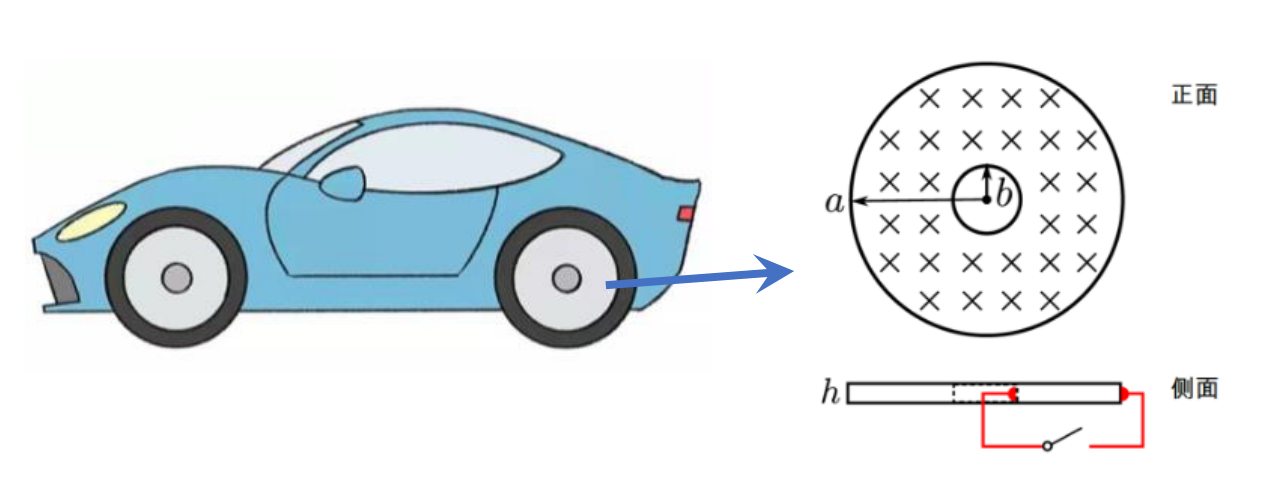
\includegraphics[width=\linewidth]{sample_brake.png}
\end{column}
\begin{column}{0.66\textwidth}
车轮半径 $r$，盘的内外半径 $b$、$a$，厚度 $h$，电阻率 $\rho$，磁场 $B$ 垂直盘面。纯滚动时 $\omega=v/r$。忽略外接电阻、自感和轮子转动惯量。径向薄环串联，截面积是 $2\pi sh$：
\[
 R=\frac{\rho}{2\pi h}\ln\frac{a}{b},\qquad
 \mathcal{E}=\frac{B(a^2-b^2)}{2r}\,v.
\]
$\vct\omega$ 与 $\vct B$ 同向时外缘电势高。功率 $P=\mathcal{E}^2/R=kv^2$，
\[
 k=\frac{B^2(a^2-b^2)^2}{4r^2R}.
\]
$h$ 越大，电阻越小。
\end{column}
\end{columns}
\src{往年期中考试样卷第4题(1)(2)(3)。}
\end{frame}

\begin{frame}{刹车距离}
题目规定，损失的动能都变成焦耳热，车辆质量为 $M$：
\[
 -\frac{\dd}{\dd t}\!\left(\frac12 Mv^2\right)=kv^2,
 \qquad M\dot v=-kv.
\]
\[
 v=v_0\e^{-t/\tau},\qquad \tau=\frac{M}{k},
 \qquad s=\tau(v_0-v_1).
\]
题设 $r=0.25\unit{m}$，$a=0.20\unit{m}$，$b=0.05\unit{m}$，$h=0.02\unit{m}$，$\rho=10^{-8}\,\Omega\cdot\mathrm{m}$，$B=0.1\unit{T}$，$M=2000\unit{kg}$。
\[
 R=1.103\times10^{-7}\,\Omega,\qquad
 k=509.9\,\mathrm{kg\,s^{-1}},\qquad
 \tau=3.922\unit{s}.
\]
从 $100$ 降到 $10$，单位是 $\mathrm{km\cdot h^{-1}}$，
\[
 t=\tau\ln 10=9.03\unit{s},\qquad
 s=\boxed{98.1\unit{m}}.
\]
速度越低，制动力越弱。这个模型里速度降到零要无限长时间，滑行距离趋近 $\tau v_0$。
\src{样卷第4题(4)(5)。$s=\tau(v_0-v_1)$ 中速度用 $\mathrm{m\,s^{-1}}$。}
\end{frame}

\begin{frame}{自感}
线圈中的电流变化时，它自己的磁通也变化，由此产生的电动势叫做自感电动势。我们可以定义磁通匝链数$Psi$等于各匝磁通之和，且有：
\[
 \Psi=LI,\qquad
 \mathcal{E}=-L\frac{\dd I}{\dd t}.
\]
$L$ 叫做自感系数。它由线圈的形状、匝数和介质决定，与电流无关。有铁磁质时 $B$ 与 $I$ 不成正比，$L$ 还随电流变化，$L$一般很难计算 。

计算时先由电流求 $\vct B$，再对每一匝积分磁通，相加得到 $\Psi$，然后 $L=\Psi/I$。

长直螺线管长 $l$，截面积 $S$，总匝数 $N$，管内 $B=\muo NI/l$，管外磁场忽略，
\[
 \boxed{L=\muo\frac{N^2S}{l}}.
\]
$l$ 不远大于半径时，两端漏磁，实际自感比这个值小。单位长度的自感是 $\muo n^2S$，$n=N/l$。
\src{张讲义第8.3节，式(8.46)及长直螺线管例题；DC7。}
\end{frame}

\begin{frame}{互感}
线圈 1 的电流在线圈 2 中产生磁链。线性介质、相对位置不变时
\[
 \Psi_{21}=M_{21}I_1,\qquad
 \mathcal{E}_2=-M_{21}\frac{\dd I_1}{\dd t}.
\]
$M_{21}$ 叫做互感系数。没有铁磁质时它与电流无关，并且
\[
 M_{12}=M_{21}=M.
\]
$M$ 的正负看两个回路的正向：正向取得一致时 $M>0$。只把一个回路的正向反过来，$M$ 变号。

两个空气芯长螺线管共轴、等长 $l$，截面积 $S_1<S_2$，匝数 $N_1$、$N_2$，$l$ 远大于半径。内管的磁场 $B_1=\muo N_1I_1/l$ 只分布在 $S_1$ 上，外管每一匝围住的有效面积仍是 $S_1$，
\[
 \boxed{M=\muo\frac{N_1N_2S_1}{l}}.
\]
改由外管的电流计算，内管处 $B_2=\muo N_2I_2/l$，每匝内管的面积还是 $S_1$，得到同一个 $M$。漏磁忽略时，$M/\sqrt{L_1L_2}=\sqrt{S_1/S_2}$。
\src{张讲义例8.5；DC7长螺线管的自感与互感。}
\end{frame}

\begin{frame}{磁场能量}
建立电流时，电源要克服自感电动势做功。线性介质里，一个线圈储存的磁场能量是
\[
 W_m=\int_0^I Li\,\dd i=\frac12 LI^2.
\]
两个线圈还要加上互感的功。$M$ 按前面的正向约定，
\[
 W_m=\frac12 L_1I_1^2+\frac12 L_2I_2^2+MI_1I_2.
\]
$M$ 可以为负，但整个 $W_m$ 不能为负，因此 $|M|\le\sqrt{L_1L_2}$。

同一能量也可以对场积分。各向同性线性介质中，能量密度是
\[
 w_m=\frac12\vct B\cdot\vct H=\frac{B^2}{2\mu}.
\]
对全空间积分，结果与电路公式一致。电流不好归成一个 $L$ 时，先积 $B^2/(2\mu)$，再由 $W_m=\dfrac12 LI^2$ 反解 $L$。铁磁质的磁化与历史有关，不能再用这个式子。
\src{张讲义第8.4节，式(8.55)、(8.73)；DC8。}
\end{frame}

\begin{frame}{RL电路}
\begin{columns}[T,onlytextwidth]
\begin{column}{0.24\textwidth}
\centering
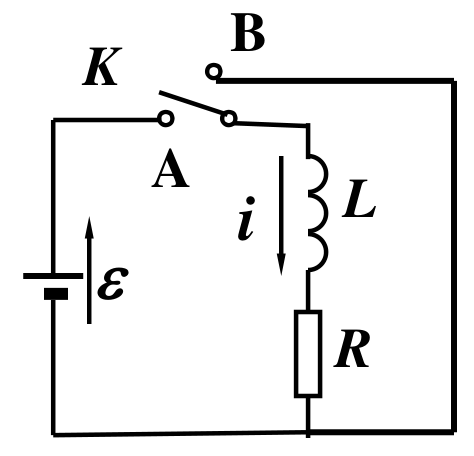
\includegraphics[width=\linewidth]{m3_RL.png}
\end{column}
\begin{column}{0.72\textwidth}
线性电感与电阻串联，时间常数 $\tau=L/R$，$R$ 含线圈电阻。电流不能突变。
\[
 L\frac{\dd i}{\dd t}+Ri=\mathcal{E}_0,\qquad
 i=\frac{\mathcal{E}_0}{R}\bigl(1-\e^{-t/\tau}\bigr).
\]
接通前电流为零。电源功率分成电阻发热和磁场能量的增加：
\[
 \mathcal{E}_0 i=Ri^2+\frac{\dd}{\dd t}\!\left(\frac12 Li^2\right).
\]
\end{column}
\end{columns}
开关改接到电阻上，初电流为 $I_0$ 时 $i=I_0\e^{-t/\tau}$，放出的热量等于 $\dfrac12 LI_0^2$。直流稳定后 $\dd i/\dd t=0$，理想电感两端电压为零。
\src{DC7，RL暂态；张讲义自感电动势与磁能。}
\end{frame}

\begin{frame}{位移电流}
稳恒时 $\nabla\times\vct H=\vct J_f$。两边取散度，得到 $\nabla\cdot\vct J_f=0$。电荷若在某处积累，连续性方程是
\[
 \nabla\cdot\vct J_f+\frac{\partial\rho_f}{\partial t}=0,
\]
与上面的结论矛盾。又因为 $\nabla\cdot\vct D=\rho_f$，所以可以引入位移电流
\[
 \nabla\cdot\!\left(\vct J_f+\frac{\partial\vct D}{\partial t}\right)=0.
\]
安培环路改成
\[
 \boxed{\nabla\times\vct H
 =\vct J_f+\frac{\partial\vct D}{\partial t}},
 \qquad
 \vct J_d\equiv\frac{\partial\vct D}{\partial t}.
\]
$\vct J_d$ 叫做位移电流密度。通过一个曲面的位移电流是 $I_d=\int\vct J_d\cdot\dd\vct S$。真空中 $\vct J_d=\epso\partial\vct E/\partial t$。

它描述变化的电场，不是电荷在导线里流动。电容器充电时，导线里有传导电流，极板之间没有；不写 $\vct J_d$，同一个环路会因所选曲面不同而得到不同的环流。补上以后，穿过导线的传导电流和穿过极板间隙的位移电流相等。
\src{张讲义第9.1节，式(9.2)--(9.5)；DC10；缪讲义8.1。}
\end{frame}

\begin{frame}{e.g,4.2费曼圆形电容器}
圆形平行板半径 $a$，间距 $d$，且 $d\ll a$，忽略边缘效应。两端接交变电压 $V=V_0\cos\omega t$。板间电场沿轴线。尺寸远小于波长时，按 $(\omega r/c)^2$ 逐级计算。

零阶先不计磁场。电场由电压决定，板间近似均匀，
\[
 E_z^{(0)}=\frac{V_0}{d}\cos\omega t.
\]
这个电场的变化率就是位移电流。$r<a$ 时，半径 $r$ 的环路围住 $\pi r^2$ 上的位移电流，
\[
 B_\varphi^{(1)}
 =-\frac{\muo\epso\omega r}{2}\frac{V_0}{d}\sin\omega t
 =-\frac{\omega r}{2c^2}\frac{V_0}{d}\sin\omega t.
\]
$r>a$ 时，位移电流只通过半径 $a$ 的圆面，$B_\varphi$ 按 $a^2/r$ 减小。

零阶电场是静电场的结果。磁场比它多一个因子 $\omega r/c^2$，是下一级小量。下面只用板间的 $B_\varphi^{(1)}$ 去修正电场。
\src{费曼物理学讲义第二卷，交变电压下的圆形电容器。}
\end{frame}

\begin{frame}{e.g,4.3费曼圆形电容器}
包含轴线的小矩形回路上，磁通来自 $B_\varphi$，因此 $\partial E_z/\partial r=\partial B_\varphi/\partial t$。代入上一级磁场，并把轴上的修正取为零：
\[
 \begin{aligned}
 E_z^{(2)}
 &=-\frac14\left(\frac{\omega r}{c}\right)^2\frac{V_0}{d}\cos\omega t,\\
 E_z^{(4)}
 &=\frac{1}{64}\left(\frac{\omega r}{c}\right)^4\frac{V_0}{d}\cos\omega t.
 \end{aligned}
\]
二阶电场的位移电流再产生磁场，这个磁场再用法拉第定律给出四阶电场。每一级都比上一级多 $(\omega r/c)^2$。$a$ 远小于波长时，二阶已经很小，板间可以用均匀的零阶电场。

\src{费曼物理学讲义第二卷，圆形电容器的逐级近似。这里不把级数收成贝塞尔函数。}
\end{frame}

\begin{frame}{麦克斯韦方程组}
自由电荷密度为 $\rho_f$，传导电流密度为 $\vct J_f$：
\begin{columns}[T,onlytextwidth]
\begin{column}{0.58\textwidth}
\textbf{积分形式}
\[
 \begin{aligned}
 \oiint\vct D\cdot\dd\vct S&=Q_{f,{\rm in}}\\
 \oiint\vct B\cdot\dd\vct S&=0\\
 \oint\vct E\cdot\dd\vct l
 &=-\frac{\dd}{\dd t}\int\vct B\cdot\dd\vct S\\
 \oint\vct H\cdot\dd\vct l
 &=I_{f,{\rm in}}+\frac{\dd}{\dd t}\int\vct D\cdot\dd\vct S
 \end{aligned}
\]
\end{column}
\begin{column}{0.40\textwidth}
\textbf{微分形式}
\[
 \begin{aligned}
 \nabla\cdot\vct D&=\rho_f\\
 \nabla\cdot\vct B&=0\\
 \nabla\times\vct E&=-\partial_t\vct B\\
 \nabla\times\vct H
 &=\vct J_f+\partial_t\vct D
 \end{aligned}
\]
\end{column}
\end{columns}
介质的本构关系不假定线性：
\[
 \vct D=\epso\vct E+\vct P,\qquad
 \vct B=\muo(\vct H+\vct M).
\]
$\vct P$、$\vct M$ 由介质和它的历史决定，不必与场成正比。
\src{张讲义第9.2节；DC10。$\vct D$、$\vct B$ 的定义不要求线性介质。}
\end{frame}

\begin{frame}{边值关系}
界面两侧分别记为 1 和 2，$\hat{\vct n}$ 从 1 指向 2。界面上自由面电荷为 $\sigma_f$，自由面电流为 $\vct K_f$。场在界面附近保持有限时，
\[
 \begin{aligned}
 \hat{\vct n}\cdot(\vct D_2-\vct D_1)&=\sigma_f,\\
 \hat{\vct n}\cdot(\vct B_2-\vct B_1)&=0,\\
 \hat{\vct n}\times(\vct E_2-\vct E_1)&=0,\\
 \hat{\vct n}\times(\vct H_2-\vct H_1)&=\vct K_f.
 \end{aligned}
\]
法向的 $\vct D$、$\vct B$ 来自高斯型的两个方程，用扁柱面。切向的 $\vct E$、$\vct H$ 来自环路型的两个方程，用跨在界面上的窄矩形。时间变化的通量在扁柱和窄矩形上是高阶小量，所以这四式对静场和时变场都用。

自由面电荷使法向 $\vct D$ 跳变，自由面电流使切向 $\vct H$ 跳变。没有自由面电荷和自由面电流时，法向 $\vct B$、$\vct D$ 连续，切向 $\vct E$、$\vct H$ 连续。电磁波在介质表面的反射和折射就用这一组。
\src{张讲义界面条件与第9.2节；DC10。}
\end{frame}

\begin{frame}{电磁场的能量}
电动力学里，场对介质做的元功密度是
\[
 \delta w=\vct E\cdot\delta\vct D+\vct H\cdot\delta\vct B.
\]
这里不要求 $\vct D$、$\vct B$ 与 $\vct E$、$\vct H$ 成正比。

线性、无色散、无磁滞时，沿场从零建立的过程积分，得到能量密度
\[
 u=\frac12\vct E\cdot\vct D+\frac12\vct B\cdot\vct H
 =\frac12\varepsilon E^2+\frac12\mu H^2.
\]
\src{张讲义第9.4节，式(9.77)--(9.79)。元功 $\vct E\cdot\delta\vct D+\vct H\cdot\delta\vct B$ 不依赖线性假设。}
\end{frame}

\begin{frame}{坡印廷矢量}
由 $\nabla\times\vct E=-\partial\vct B/\partial t$ 和 $\nabla\times\vct H=\vct J_f+\partial\vct D/\partial t$，在线性无色散介质中得到
\[
 \boxed{\frac{\partial u}{\partial t}+\nabla\cdot\vct S
 =-\vct J_f\cdot\vct E},
 \qquad
 \boxed{\vct S=\vct E\times\vct H}.
\]
$\vct S$ 叫做坡印廷矢量，方向是电磁能量流动的方向，大小是单位时间通过垂直于该方向的单位面积的能量。

对固定体积积分，边界外法向为 $\dd\vct A$，
\[
 -\oiint\vct S\cdot\dd\vct A
 =\frac{\dd}{\dd t}\int u\,\dd V
 +\int\vct J_f\cdot\vct E\,\dd V.
\]
左边是单位时间流入这个体积的电磁能量。右边第一项是场能的增加，第二项是场对电流做功的功率，相当于焦耳热。
稳恒时场能不变，流入的功率等于焦耳热。没有电流时，流入的功率等于场能的增加率。
\src{张讲义第9.4节，式(9.84)--(9.92)；DC10。}
\end{frame}

\begin{frame}{电阻中的能流}
\begin{columns}[T,onlytextwidth]
\begin{column}{0.68\textwidth}
圆柱电阻长 $L$、半径 $a$，两端电压 $U$，稳恒电流 $I$ 沿 $+z$。柱内
\[
 E_z=\frac{U}{L},\qquad
 H_\varphi(a)=\frac{I}{2\pi a}.
\]
侧面的坡印廷矢量指向轴，
\[
 \vct S(a)=-\frac{UI}{2\pi a L}\vct e_r.
\]
从整个侧面流入的功率是
\[
 P=-\int\vct S\cdot\dd\vct A=UI.
\]
\end{column}
\begin{column}{0.28\textwidth}
\centering
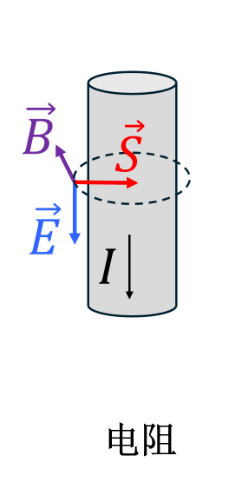
\includegraphics[height=4.2cm]{m4_resistor_energy_flow.png}
\end{column}
\end{columns}
电能从侧面进入导体，变成焦耳热。电场和磁场都可以不随时间变化。$H_\varphi$ 用柱面外缘的安培环路；电流均匀时，内部任一圆柱侧面流入的功率等于该圆柱内的焦耳热。
\src{张讲义坡印廷矢量的电阻例子；DC10；教材习题10.7。}
\end{frame}

\begin{frame}{电磁场的动量}
真空中，电磁场的动量密度是
\[
 \boxed{\vct g=\epso\vct E\times\vct B=\frac{\vct S}{c^2}}.
\]
$\vct S$ 沿能量传播的方向，动量也沿这个方向。一段真空中的波若携带能量 $U$，它的动量大小就是 $U/c$。

波垂直射到不透明的表面上，入射强度为 $I$，照射面积为 $A$。单位时间入射的能量是 $IA$，带来的动量是 $IA/c$。全部被吸收时，交给表面的动量就是这些，压强为 $I/c$。全部被垂直反射时，反射波带走相反的动量，表面得到的动量是入射的两倍，压强为 $2I/c$。反射率是 $R$、其余都被吸收时，压强是 $(1+R)I/c$。

介质里动量密度有不止一种写法。一般考试也不会考（除非出卷人相对恶意）
\src{张讲义第9.4节；DC10；教材第10章。}
\end{frame}

\begin{frame}{光压}
光强为 $I$，光线与平面法线的夹角为 $\theta$，镜面的实际面积为 $A$，镜面不透光。单位时间射到镜面上的能量是 $IA\cos\theta$，因为光束的横截面积是 $A\cos\theta$。

动量沿光线方向。全反射时，法向动量的改变还要再乘一个 $\cos\theta$，法向压强是
\[
 \boxed{p_n=\frac{2I}{c}\cos^2\theta}.
\]
吸收的份额为 $\alpha$，其余仍按镜面反射时，
\[
 p_n=\frac{(2-\alpha)I}{c}\cos^2\theta.
\]
被吸收的那一部分动量沿原来的光线，所以还有切向力。单位面积上的切向力是 $\alpha I\sin\theta\cos\theta/c$。

\src{期中复习笔记题10.9；教材习题10.9；张讲义光压。}
\end{frame}

\begin{frame}{电磁场的角动量}
相对于原点，真空中电磁场的角动量密度和总角动量是
\[
 \vct\ell=\vct r\times\vct g,
 \qquad
 \vct L=\int\vct r\times(\epso\vct E\times\vct B)\,\dd V.
\]
$\vct g$ 沿方位角、$\vct r$ 沿径向时，$\vct\ell$ 沿轴线。径向电场和轴向磁场叠在一起，就是这种情形。

没有外力矩时，机械角动量与场的角动量之和守恒。外力矩的冲量等于两者之和的增加。

积分范围要包括电场和磁场同时不为零的全部区域。带电圆柱面的磁场常常在柱内，电场常常在柱外，角动量就在柱面外面。只对柱面内部积分，结果可以是零。
\src{DC10；教材电磁场的动量与角动量。介质中的动量不采用 $\vct S/c^2$。}
\end{frame}

\begin{frame}{e.g.5带电圆柱面加速}
两个共轴无限长圆柱面，半径 $a<b$。内柱单位长度电荷 $+\lambda$，外柱单位长度电荷 $-\lambda$。外力使两层以同一个角速度 $\omega(t)$ 绕轴线加速，$\omega$ 沿 $+z$。下面先不计圆柱面自己的转动惯量，外力矩只用来改变电磁场。

电荷随柱面转动，形成沿方位角的面电流
\[
 K_a=\frac{\lambda\omega}{2\pi},\qquad
 K_b=-\frac{\lambda\omega}{2\pi}.
\]
每一层都相当于一个螺线管，磁场只在该层以内。两层叠加：
\[
 B_z=
 \begin{cases}
 0,&r<a,\\
 -\muo\lambda\omega/(2\pi),&a<r<b,\\
 0,&r>b.
 \end{cases}
\]
静电场只在两层之间，$E_r=\lambda/(2\pi\epso r)$。内柱里面和外柱外面，静电场都是零。

因此 $\vct E$ 和 $\vct B$ 只在 $a<r<b$ 同时存在。这个区域在内柱面的外面。
\src{无限长带电圆柱面的电场、等效螺线管磁场。以下三页用同一模型。}
\end{frame}

\begin{frame}{e.g.5带电圆柱面加速-力矩法}
$\omega$ 增大时，只有 $a<r<b$ 的磁通在变。环路正向与 $+z$ 成右手关系，$a<r<b$ 时
\[
 \Phi_B=B_z\,\pi(r^2-a^2)
 =-\frac{\muo\lambda\omega}{2}(r^2-a^2).
\]
\[
 E_\varphi=\frac{\muo\lambda\dot\omega\,(r^2-a^2)}{4\pi r}.
\]
内柱面 $r=a$ 上 $E_\varphi=0$，感生电场对内柱面没有力矩。外柱面
\[
 E_\varphi(b)=\frac{\muo\lambda\dot\omega\,(b^2-a^2)}{4\pi b}.
\]
外柱面单位长度电荷是 $-\lambda$，受力与 $E_\varphi$ 相反，力矩沿 $-z$，阻碍加速。单位长度上，这个力矩的大小是
\[
 \tau=\frac{\muo\lambda^2(b^2-a^2)}{4\pi}\dot\omega.
\]
忽略转动惯量时，外力矩与它平衡，方向沿 $+z$，大小就是 $\tau$。电磁力矩加在外柱面上，不加在内柱面上。
\src{法拉第定律与洛伦兹力。环路正向与 $+z$ 成右手系。}
\end{frame}

\begin{frame}{e.g.5带电圆柱面加速-角动量法}
动量密度 $\vct g=\epso\vct E\times\vct B$。$a<r<b$ 中 $\vct E$ 沿径向，$\vct B$ 沿 $-z$，所以 $\vct g$ 沿方位角。角动量密度沿 $+z$，并且与 $r$ 无关：
\[
 \ell_z=\frac{\muo\lambda^2\omega}{4\pi^2}.
\]
对 $a<r<b$ 的圆环面积积分，单位长度的角动量是
\[
 \boxed{L_z=\frac{\muo\lambda^2\omega(b^2-a^2)}{4\pi}}.
\]
$r<a$ 时电场和磁场都是零，$r>b$ 时也是零，这两处的贡献都是零。$L_z$ 全部在内柱面之外、外柱面之内。

只对内柱面内部积分，得到的角动量是零，它的变化率也是零，和外力矩 $\tau$ 对不上。对 $a<r<b$ 积分以后，
\[
 \frac{\dd L_z}{\dd t}=\tau.
\]
外力矩的冲量等于场的角动量的增加。
\src{真空动量密度 $\epso\vct E\times\vct B$。角动量必须含 $a<r<b$。}
\end{frame}

\begin{frame}{e.g.5带电圆柱面加速-能量法}
磁场只在 $a<r<b$。单位长度的磁场能量是
\[
 U=\frac{B^2}{2\muo}\,\pi(b^2-a^2)
 =\frac{\muo\lambda^2\omega^2(b^2-a^2)}{8\pi}.
\]
外力矩的功率
\[
 \tau\omega=\frac{\muo\lambda^2\omega\dot\omega\,(b^2-a^2)}{4\pi}
 =\frac{\dd U}{\dd t}.
\]
外力做的功全部变成磁场能量。静电场的能量与 $\omega$ 无关，不进入这个功率。

感生电场的力矩、场的角动量、磁场能量，给出的是同一个外力矩
\[
 \tau=\frac{\muo\lambda^2(b^2-a^2)}{4\pi}\dot\omega.
\]
圆柱面自己还有转动惯量 $I_a$、$I_b$ 时，外力矩要再加上 $(I_a+I_b)\dot\omega$。多出来的这一部分只增加机械角动量和动能，不改变上面的磁场能量和场的角动量。
\src{三种算法：感生电场的力矩、角动量守恒、磁场能量。}
\end{frame}

\begin{frame}{波动方程}
均匀、各向同性、不导电的介质，$\varepsilon$ 和 $\mu$ 都是常数，并且没有自由电荷和传导电流。麦克斯韦方程写成
\[
 \nabla\cdot\vct E=0,\qquad
 \nabla\times\vct E=-\mu\frac{\partial\vct H}{\partial t},\qquad
 \nabla\times\vct H=\varepsilon\frac{\partial\vct E}{\partial t}.
\]
对第二式取旋度，把第三式代进去，再用
\[
 \nabla\times(\nabla\times\vct E)
 =\nabla(\nabla\cdot\vct E)-\nabla^2\vct E,
\]
得到
\[
 \boxed{\nabla^2\vct E
 =\mu\varepsilon\frac{\partial^2\vct E}{\partial t^2}},
 \qquad
 v=\frac{1}{\sqrt{\mu\varepsilon}}.
\]
$\vct H$ 满足同一个方程。真空中 $c=1/\sqrt{\muo\epso}$。

推导里用了 $\nabla\cdot\vct E=0$，也没有传导电流。若 $\vct J=\sigma\vct E$，或 $\varepsilon$ 随频率变化，方程改成亥姆霍兹方程，波会衰减，波速也与频率有关。
\src{张讲义第9.3节，式(9.43)--(9.51)；DC10。}
\end{frame}

\begin{frame}{平面波}
沿 $\vct k$ 传播的单色平面波，
\[
 \vct E=\vct E_0\cos(\vct k\cdot\vct r-\omega t),
 \qquad k=\frac{\omega}{v}.
\]
代入无源的麦克斯韦方程，
\[
 \vct k\cdot\vct E=0,\qquad
 \vct k\cdot\vct B=0,\qquad
 \vct B=\frac1v\hat{\vct k}\times\vct E.
\]
\[
 \vct H=\frac1Z\hat{\vct k}\times\vct E,
 \qquad
 Z=\sqrt{\frac{\mu}{\varepsilon}}.
\]
$\vct E$、$\vct H$ 和传播方向两两垂直，三者成右手关系。无损耗介质中的行波里，$\vct E$ 和 $\vct H$ 同相，振幅满足 $E_0=ZH_0=vB_0$。

真空波阻抗 $Z_0=\sqrt{\muo/\epso}\simeq377\,\Omega$。一个周期内的平均能流沿传播方向，大小是
\[
 I=\langle S\rangle=\frac{E_0H_0}{2}=\frac{E_0^2}{2Z}.
\]
$E_0$、$H_0$ 是峰值，有效值再除以 $\sqrt2$。
\src{张讲义第9.3节，式(9.60)--(9.76)；DC10。}
\end{frame}

\begin{frame}{介质中的电磁波}
线性无损耗介质中，波速、折射率和波阻抗是
\[
 v=\frac{1}{\sqrt{\mu\varepsilon}},\qquad
 n=\frac{c}{v}=\sqrt{\varepsilon_r\mu_r},\qquad
 Z=\sqrt{\frac{\mu}{\varepsilon}}.
\]
非磁介质 $\mu_r=1$，于是 $n=\sqrt{\varepsilon_r}$，$v=c/n$，$Z=Z_0/n$。折射率越大，波越慢，波阻抗越小。

平面行波的关系仍然是 $\vct B=\hat{\vct k}\times\vct E/v$，$\vct H=\hat{\vct k}\times\vct E/Z$。电场能量密度和磁场能量密度相等，总能量密度 $u=\varepsilon E^2$，能流 $\vct S=uv\hat{\vct k}$。

\src{张讲义第9.6节；缪讲义介质中的电磁波。}
\end{frame}

\begin{frame}{界面上的电磁波}
介质界面上没有自由面电荷，也没有自由面电流。边值关系变成：法向 $\vct B$、法向 $\vct D$ 连续，切向 $\vct E$、切向 $\vct H$ 连续。

设界面是 $z=0$，入射、反射、折射三列波在界面上要每一点、每一时刻都接得上，所以三列波的频率相同，波矢的切向分量相同。由此得到三列波的波矢在同一平面内，并且
\[
 \theta_r=\theta_i,\qquad
 n_1\sin\theta_i=n_2\sin\theta_t.
\]
第一式是反射定律，第二式是折射定律。$\theta$ 都是波矢与法线的夹角。

频率相同，是因为边界条件要对所有时刻成立。切向波矢相同，是因为边界条件要对界面上所有点成立。角度关系只来自这一条，与偏振无关。振幅还要再用切向 $\vct E$、$\vct H$ 来定。
\src{张讲义第9.7节，式(9.170)--(9.176)。}
\end{frame}

\begin{frame}{菲涅尔公式}
垂直入射时，入射波和透射波的电场沿同一方向取正。反射波传播方向相反，磁场相对电场也反过来。切向电场、切向磁场连续：
\[
 E_i+E_r=E_t,\qquad
 \frac{E_i-E_r}{Z_1}=\frac{E_t}{Z_2}.
\]
\[
 \boxed{r=\frac{E_r}{E_i}=\frac{Z_2-Z_1}{Z_2+Z_1}},
 \qquad
 \boxed{t=\frac{E_t}{E_i}=\frac{2Z_2}{Z_2+Z_1}}.
\]
非磁介质 $Z=Z_0/n$，
\[
 r=\frac{n_1-n_2}{n_1+n_2},\qquad
 t=\frac{2n_1}{n_1+n_2}.
\]
平均能流 $I=E_0^2/(2Z)$。能量反射率和能量透射率是
\[
 R=r^2,\qquad
 T=\frac{Z_1}{Z_2}t^2,\qquad R+T=1.
\]
波阻抗小的一侧，同样的电场对应更大的能流，所以透射能量比带有 $Z_1/Z_2$。
\src{张讲义式(9.197)--(9.216)；缪讲义介质表面；样卷第5题(1)(2)。}
\end{frame}

\begin{frame}{斜入射}
非磁介质，电场垂直于入射面时，切向电场就是 $E$ 本身，切向磁场带有 $\cos\theta$。仍取同一电场正向，
\[
 E_i+E_r=E_t,
\]
\[
 n_1(E_i-E_r)\cos\theta_i=n_2 E_t\cos\theta_t.
\]
\[
 r_s=\frac{n_1\cos\theta_i-n_2\cos\theta_t}
 {n_1\cos\theta_i+n_2\cos\theta_t},\qquad
 t_s=\frac{2n_1\cos\theta_i}
 {n_1\cos\theta_i+n_2\cos\theta_t}.
\]
电场在入射面内时，切向电场带有 $\cos\theta$，磁场垂直于入射面：
\[
 r_p=\frac{n_2\cos\theta_i-n_1\cos\theta_t}
 {n_2\cos\theta_i+n_1\cos\theta_t},\qquad
 t_p=\frac{2n_1\cos\theta_i}
 {n_2\cos\theta_i+n_1\cos\theta_t}.
\]
垂直入射时两种偏振的能量反射率相同。$r_p$ 和 $r_s$ 差一个符号，来自反射波电场正向的取法。用同一切向坐标取正负时，垂直入射的反射系数回到 $(n_1-n_2)/(n_1+n_2)$。

能量反射率仍是 $r^2$。斜入射的能量透射率还要乘 $\cos\theta_t/\cos\theta_i$，因为折射光束的横截面积和入射光束不同。
\src{张讲义第9.7节菲涅尔公式。非磁介质，$\mu_1=\mu_2=\muo$。}
\end{frame}

\begin{frame}{垂直入射}
\begin{columns}[T,onlytextwidth]
\begin{column}{0.66\textwidth}
平面波从真空垂直射入非磁介质，折射率 $n=\sqrt{\varepsilon/\epso}$，波阻抗 $Z=Z_0/n$。由垂直入射的菲涅尔公式，
\[
 E_r=\frac{1-n}{1+n}E_i,\qquad
 E_t=\frac{2}{1+n}E_i.
\]
平均能流 $I_i=E_i^2/(2Z_0)$，$I_r=E_r^2/(2Z_0)$，$I_t=nE_t^2/(2Z_0)$。
\[
 R=\frac{(1-n)^2}{(1+n)^2},\qquad
 T=\frac{4n}{(1+n)^2},\qquad
 R+T=1.
\]
$n>1$ 时反射电场反向。相同截面上，入射功率等于反射功率与透射功率之和。
\end{column}
\begin{column}{0.30\textwidth}
\centering
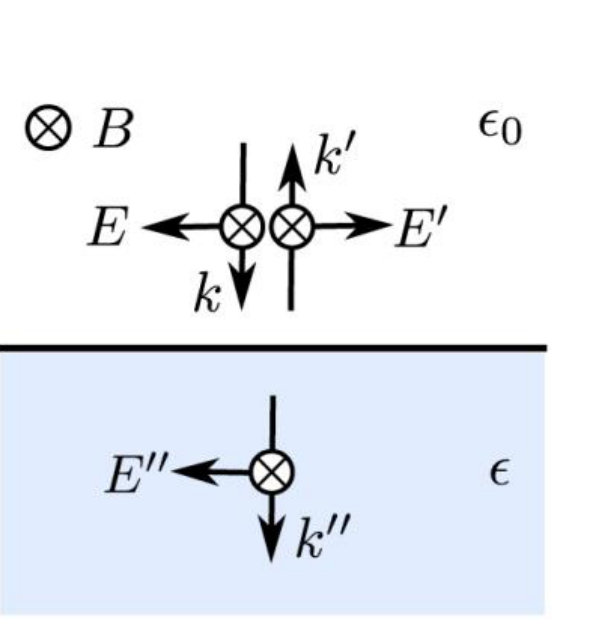
\includegraphics[width=\linewidth]{sample_normal_wave.png}
\end{column}
\end{columns}
$n=1.50$ 时 $r=-0.20$，$t=0.80$，$R=0.04$，$T=0.96$。透射电场是入射的 $0.8$ 倍，透射能量占 $96\%$，因为介质一侧的波阻抗更小。
\src{样卷第5题(1)(2)；缪讲义介质表面。无损介质。}
\end{frame}

\begin{frame}{导体中的电磁波-震荡模型}
均匀导体里，正离子不动。忽略碰撞和回复力时，自由电子数密度为 $N$，电场 $E=E_0\cos\omega t$ 使电子的位移为
\[
 x=\frac{eE}{m_e\omega^2}.
\]
极化强度 $P=-Nex$，于是
\[
 \boxed{\varepsilon(\omega)
 =\epso\!\left(1-\frac{\omega_p^2}{\omega^2}\right)},
 \qquad
 \omega_p=\sqrt{\frac{Ne^2}{\epso m_e}}.
\]
$\omega>\omega_p$ 时 $\varepsilon>0$，波可以传播。$\omega<\omega_p$ 时 $\varepsilon<0$，
\[
 k=\ii\kappa,\qquad
 \kappa=\frac{\sqrt{\omega_p^2-\omega^2}}{c}.
\]
电场在表面内按 $\e^{-\kappa z}$ 衰减，磁场与电场相位差 $\pi/2$，平均能流为零。半无限厚又无碰撞时，能量反射率为 $1$。有碰撞时，低频导体以欧姆电导为主。
\src{缪讲义等离子体频率；样卷第5题(3)(4)。}
\end{frame}

\begin{frame}{导体中的电磁波-震荡模型}
金属电子数密度 $N=10^{28}\,\mathrm{m^{-3}}$，波长 $\lambda=500\,\mathrm{nm}$，金属占满半无限空间，仍忽略碰撞。
\[
 \omega_p=\sqrt{\frac{Ne^2}{\epso m_e}}
 =5.64\times10^{15}\unit{s^{-1}},
\]
\[
 \omega=\frac{2\pi c}{\lambda}
 =3.77\times10^{15}\unit{s^{-1}}.
\]
$\omega<\omega_p$，
\[
 \varepsilon_r=1-\frac{\omega_p^2}{\omega^2}\simeq-1.24,
 \qquad
 \kappa\simeq1.40\times10^{7}\unit{m^{-1}}.
\]
场在大约 $1/\kappa=72\unit{nm}$ 内衰减，能量反射率 $R=1$。这束绿光被金属全反射，没有净能流进入金属深处。

判断顺序是：先比较 $\omega$ 和 $\omega_p$，再看 $\varepsilon$ 的符号。$\varepsilon<0$ 时 $k$ 为虚数，无碰撞的半无限金属把入射能量全部反射。
\src{样卷第5题(4)。$e=1.60\times10^{-19}\unit{C}$，$m_e=9.11\times10^{-31}\unit{kg}$，$\epso=8.85\times10^{-12}\,\mathrm{F\,m^{-1}}$。}
\end{frame}

\begin{frame}{导体中的电磁波-电导模型}
导体里更常用的做法是直接写 $\vct J=\sigma\vct E$。单色场取 $\e^{-\ii\omega t}$ 时，
\[
 \nabla\times\vct H=\sigma\vct E-\ii\omega\varepsilon\vct E,
 \qquad
 \nabla\times\vct E=\ii\omega\mu\vct H.
\]
消去 $\vct H$。均匀导体内部 $\nabla\cdot\vct E=0$，得到亥姆霍兹方程
\[
 \boxed{\nabla^2\vct E+k^2\vct E=0},
 \qquad
 k^2=\mu\varepsilon\omega^2+\ii\mu\sigma\omega.
\]
也可写成 $k^2=\mu\varepsilon_c\omega^2$，$\varepsilon_c=\varepsilon+\ii\sigma/\omega$。$\sigma$ 是给定的常数，不需要再从电子运动求介电函数。

良导体 $\sigma\gg\omega\varepsilon$ 时，$k^2\approx\ii\mu\sigma\omega$，
\[
 k=\frac{1+\ii}{\delta},\qquad
 \delta=\sqrt{\frac{2}{\mu\sigma\omega}}.
\]
沿 $+z$ 传播的场按 $\e^{-z/\delta}$ 衰减。$\delta$ 是趋肤深度。$\sigma$ 越大、频率越高，波进入导体越浅。
\src{由 $\vct J=\sigma\vct E$ 代入安培--麦克斯韦方程。时间因子为 $\e^{-\ii\omega t}$。}
\end{frame}

\begin{frame}{发射功率}
某广播电台希望在 $100\,\mathrm{km}$ 外，信号电场的振幅不小于 $0.10\,\mathrm{V\,m^{-1}}$。求发射功率至少要多大。

按真空、各方向发射相同、没有传播损耗来估计。远处一小块波面用平面波的平均能流 \(I=E_0^2/(2Z_0)\)。

Z0是真空波阻抗的数值。由 \(c=1/\sqrt{\muo\epso}\)，
\[
 Z_0=\sqrt{\frac{\muo}{\epso}}=\muo c.
\]
取 \(\muo=4\pi\times10^{-7}\)、\(c=3.00\times10^{8}\)，得到 \(Z_0=120\pi\simeq377\,\Omega\)。

这些功率铺在半径 $r$ 的整个球面上，
\[
 \boxed{P_{\min}=4\pi r^2 I
 =\frac{2\pi r^2 E_0^2}{Z_0}
 \simeq1.67\times10^{6}\,\mathrm{W}}.
\]
距离加倍，或要求的振幅加倍，功率都变为四倍。
\src{张讲义习题9.3。}
\end{frame}
